\documentclass[preprint,review,12pt]{elsarticle}
\usepackage[T1]{fontenc}
\usepackage{amsmath,amssymb,booktabs,graphicx,xcolor,multirow}
\usepackage{tikz}
\usetikzlibrary{arrows.meta,decorations.pathreplacing}
\usepackage[hidelinks]{hyperref}
\newcommand{\pending}[1]{{\color{orange!75!black}\textsf{\small[#1]}}}
\newcommand{\FAR}{\mathrm{FAR}}
\newcommand{\DR}{\mathrm{DR}}
\journal{Computer Networks}
\setlength{\emergencystretch}{2em}

\begin{document}
\begin{frontmatter}

\title{Warning before the link degrades: evaluating radio-quality forecasts as preventive actions under a false-alarm budget}

\author{David Olutunde Daniel}
\ead{dod220001@utdallas.edu}
\address{Department of Mathematical Sciences, The University of Texas at Dallas, 800 W.\ Campbell Rd, Richardson, TX 75080, United States; and AT\&T Chief Data Office, Dallas, TX, United States}

\begin{abstract}
Proactive mobility management needs rare, timely warnings of radio link degradation.
Forecasters are usually compared by sample-level accuracy, which does not say how many
degradations are warned at an affordable false-alarm rate. We specify warning as
preventive actions, each valid for a horizon $H$ and charged when issued or renewed,
and evaluate predictors offline by the share of degradation onsets warned and false
actions per exposure hour on links used neither for fitting nor for setting the alarm
threshold, after checking the specification against uninformed policies. On public
drive-test traces from Cork, Ireland (5G non-standalone, with LTE-anchor measurements,
and 4G), learned forecasters have higher AUPRC than received-power rules in every
setting, yet at two false actions per hour none warns about more onsets than a 3GPP
A2-style rule with time-to-trigger and hysteresis on 5G (38\% at $H=30$\,s against
30--34\%), and on 4G they add at most a few points to a low baseline. When degradation
is instead defined by delivered throughput, every predictor using serving-cell radio
measurements warns about at most 11\% of onsets at that rate, and learning adds at
most a few points. At one false action per hour at most 40\% of radio-defined onsets
are warned, and calibrated thresholds exceed their budget on new links by up to a
factor of 15. Accuracy does not predict the operational benefit of learning; standard
received-power rules evaluated under the same budget are essential baselines.
\end{abstract}

\begin{keyword}
Radio link degradation \sep proactive handover \sep early warning \sep
false-alarm budget \sep evaluation methodology \sep machine learning for networking
\end{keyword}
\end{frontmatter}

%% ===================================================================
\section{Introduction}
\label{sec:intro}

A mobile network that anticipates a degradation of a user's radio link can act
before the user notices: prepare a handover to a better cell, switch carrier,
move traffic to another radio access technology, or ask a video client to lower
its bitrate. Proactive control of this kind is central to handover management
\cite{tayyab2019,mollel2021survey,alraih2023} and is a natural application for the
control loops of open radio access networks \cite{polese2023}; conditional
handover already lets the network prepare a target cell in advance
\cite{pjanic2024}.

Every preventive action has a cost: a handover preparation reserves resources and
adds signalling, and a premature bitrate reduction lowers quality for nothing. An
operator therefore needs to know, for a candidate forecaster, how many
degradations it would warn about at the rate of wasted actions the operator can
afford, and how early. Studies of radio-quality and handover prediction mostly
report regression error or sample-level classification metrics such as AUROC,
AUPRC or F1 \cite{mollel2021,fauzi2022,mohammadjafari2020,lima2023,manalastas2023}.
Such metrics score measurements independently, do not count events, and do not
fix a false-alarm rate. Event-oriented evaluation of alarm systems has a long
history \cite{fawcett1999,lavin2015,tatbul2018}, and recent work on railway 5G
networks evaluates early warning of radio link failure over prediction horizons
\cite{chou2025}. What is still missing for degradation forecasting is an
evaluation that (i) cannot be satisfied by an uninformative policy, (ii) charges
for every preventive action, and (iii) measures performance on links that were
used neither to fit the forecaster nor to set its alarm threshold, against simple
signal-level baselines evaluated in the same way.

This paper makes three contributions.
\begin{enumerate}
\item \textbf{A specification of degradation warning as preventive actions}
(Section~\ref{sec:model}). An alarm triggers an action that claims a degradation
within $H$ seconds; a still-active alarm triggers a new action when the previous
one expires. Detection, false actions per exposure hour, alarm duty and lead
($\le H$) follow directly. Unlike counting alarm runs, this cannot be satisfied by
an always-on alarm, which we verify together with always-off, oracle and random
policies before any training.
\item \textbf{A clean protocol for unseen links} (Section~\ref{sec:design}): within
each outer cross-validation fold, the training links are split into fitting,
early-stopping and calibration links; the frozen model scores calibration and test
links, and the alarm threshold is chosen on the calibration links alone. Inputs are
strictly causal: features, imputation and the decision whether to score a moment
use only measurements up to that moment.
\item \textbf{An empirical comparison} of five signal-level rules, among them a
3GPP A2-style rule with time-to-trigger and hysteresis, an uninformed random score and
six learned predictors, including same-input ablations, on three public datasets with
different technologies, sampling and degradation frequencies, with link-level paired
bootstrap intervals, a sensitivity analysis, and a repetition with a degradation event
defined by delivered throughput instead of radio quality (Section~\ref{sec:results}).
\end{enumerate}

The findings are conditional. Every full-feature learned model has higher AUPRC than
the signal rules, but whether it warns about more degradations at a given false-alarm
rate depends on the dataset, the horizon and the rate. On Cork 5G NSA no learned model
warns about more onsets than an A2-style received-power rule at one or two false
actions per hour, and learned models and a plain received-power threshold stay within a
few points of each other, ahead or behind depending on how operating points are
compared. On Cork 4G learned models add a few points to a low detection rate, about two
over a rule that extrapolates the RSRP trend at $H=30$\,s. On the Manaus data, whose
links aggregate several devices, they add 12--26 points. When the event is defined by
delivered throughput rather than radio quality, every predictor fed with serving-cell
radio measurements warns about few onsets and learning adds little. Under
strict budgets most degradations are not warned, and thresholds chosen on
calibration links can miss their budget on new links by a large factor for every
predictor, the simple rules included.

\paragraph{Relation to earlier work by the author}
A retrospective, change-point-based lead-time measure is applied to mobile stress
sensing in a separate paper by the author \cite{daniel2026sh}. The present paper
does not use that measure; it introduces a causal, action-based specification, and
its protocol, baselines, datasets and results are distinct from that work.

%% ===================================================================
\section{Related work}
\label{sec:related}

\paragraph{Predicting radio quality and mobility events}
Machine learning has been used to predict coverage and received power
\cite{fauzi2022,mohammadjafari2020}, quality of service in operational LTE
networks \cite{mollel2021}, handovers and handover failures
\cite{lima2023,manalastas2023,pjanic2024}; surveys cover the wider use of learning
in handover management \cite{tayyab2019,mollel2021survey,alraih2023}. Chou et
al.\ \cite{chou2025} benchmark several learning models for early warning of radio
link failure on 10\,Hz measurements from a 5G non-standalone metro network,
across observation windows and prediction horizons. They report frame-level
accuracy, precision, recall and F1 at a fixed probability threshold of 0.5 on
validation data, and the share of 23 breakdown events covered under point-count and
consecutive trigger rules; they note that event-level false alarms are not quantified
and that choosing a trigger policy requires that evaluation. Relative to that study, the present paper adds the three elements listed
in Section~\ref{sec:intro}: checks that uninformed policies cannot score well, a
charge for every issued or renewed action, and thresholds calibrated on separate links
together with a measure of whether their budget holds on new links. Capacity forecasting for
network slicing faces a related asymmetry between over- and under-provisioning
\cite{bega2019}. Public drive-test datasets used here are the multi-operator
Amazonas dataset \cite{silva2024} and the Cork 4G and 5G traces
\cite{raca2018,raca2020}.

\paragraph{Evaluating alarms and early warnings}
Activity monitoring \cite{fawcett1999} evaluates an alarm system by the share of
events detected against the false-alarm rate. Streaming anomaly benchmarks reward
early detection within a window around each event and penalise false positives
\cite{lavin2015}, range-based precision and recall extend point metrics to events
with duration \cite{tatbul2018}, and sequential change detection formalises the
trade-off between detection delay and false alarms \cite{tartakovsky2014}. On
imbalanced data AUPRC is more informative than AUROC \cite{saito2015}, but both
summarise all thresholds and all samples. Leakage through features or through
evaluation that reuses test entities inflates reported performance
\cite{kaufman2012,kapoor2023}. Our contribution is not a new detection metric but
a specification and protocol that make these principles concrete and testable for
radio degradation warning, and an assessment of what they change. Event-level
detection against false alarms per unit time is the activity-monitoring view
\cite{fawcett1999}; what is specific here is charging renewals of a held alarm,
calibrating thresholds out of sample, and measuring budget transfer.

%% ===================================================================
\section{System model and problem formulation}
\label{sec:model}

\subsection{Scenario}
Each user equipment (UE) reports periodic measurements of its serving link to a
controller, for example an application in a near-real-time RAN intelligent
controller \cite{polese2023} or an operator's mobility-management function. After
each report the controller decides whether an alarm is on for that UE. An alarm
triggers a \emph{preventive action}, such as preparing a conditional handover,
switching carrier or asking the application to adapt, which remains valid for $H$
seconds. If the alarm is still on when the action expires, the controller renews it,
which is a new action with a new cost. An action followed by a degradation within its
validity is useful; any other action is wasted. The operator limits wasted actions
to a budget $\beta$ per hour of monitored link time.

\subsection{Measurement and degradation model}
Link $\ell$ (a measurement session, or for one dataset a device model on a cell;
Section~\ref{sec:data}) produces measurements at times $t_{\ell,1}<t_{\ell,2}<\cdots$,
not necessarily equally spaced, with
$\mathbf{x}_{\ell,i}=(\mathrm{RSRP},\mathrm{RSRQ},\mathrm{SINR},\mathrm{CQI})_{\ell,i}$.
A record is split into \emph{segments} wherever two consecutive measurements are
more than $G=30$\,s apart \emph{or} a measurement lacks RSRP or CQI (for example while
the UE is on 2G or 3G); nothing is computed across a segment boundary. Missing RSRQ
or SINR values are carried forward within a segment, never backward, and a missing
indicator is kept.

A measurement is \emph{degraded} if
\begin{equation}
\mathrm{RSRP}_{\ell,i}<\theta_P \quad\text{and}\quad \mathrm{CQI}_{\ell,i}<\theta_C,
\label{eq:degraded}
\end{equation}
with $\theta_P=-100$\,dBm and $\theta_C=7$: weak coverage together with a channel
that cannot sustain moderate-rate modulation. This is a study-specific proxy for
service degradation; Section~\ref{sec:proxy} checks it against delivered
throughput and Section~\ref{sec:sens} varies it. A \emph{degradation episode} is a
run of at least $m=2$ consecutive degraded measurements, and its first measurement
is an \emph{onset} if at least $c=3$ non-episode measurements precede it in the
segment. Episodes and onsets are ground truth, determined retrospectively.

\subsection{Causal eligibility and labels}
A predictor may only use what the controller knows. At time $t_{\ell,i}$ an episode
is \emph{observably under way} if the last $m$ measurements up to and including $i$
are all degraded; such moments are not scored, since there is nothing left to warn
about. Every other moment with at least $W=20$ measurements of history in the
segment is \emph{eligible}. Its label for horizon $H$ is 1 if an onset occurs in
$(t,t+H]$, 0 if the segment is observed through $t+H$ without one, and
\emph{censored} otherwise; censored moments, which occur only at the end of a
segment, are neither scored nor counted. A predictor computes a risk score
$s_{\ell,i}=f(\mathbf{x}_{\ell,i-W+1:i},\Delta\mathbf{t}_{\ell,i-W+1:i})$ from the
window that ends at the current measurement.

\subsection{Warning policy and measures}
\label{sec:measures}
A threshold $\tau$ sets the alarm $a_{\ell,i}=\mathbf{1}[s_{\ell,i}\ge\tau]$; the
alarm state holds until the next measurement and is off at ineligible moments and
segment ends. An \emph{action} fires when the alarm switches on, and again every $H$
seconds while it stays on. Action $k$ at time $a_k$ claims an onset in
$(a_k,a_k+H]$. It is \emph{true} if an onset is observed in that window, even when
the window extends past the end of the segment (the same rule that labels a moment
positive); \emph{false} if the segment is observed through $a_k+H$ without an onset;
and \emph{censored}, and not counted, if the segment ends before $a_k+H$ without an
onset. Censoring is applied retrospectively, when scoring outcomes; it never affects
when the controller raises or renews an alarm, which depends only on the causal
score stream. In the implementation, scores are stored only for eligible moments with
an observed label. This omits nothing that is counted: a moment is censored only if no
onset lies in $(t,t+H]$ and the segment ends before $t+H$, so every later eligible moment
of that segment is censored as well and has no onset ahead of it, and any action the
omitted moments would raise or renew is itself censored. A full replay over all
eligible moments, censored ones included, reproduces detection, false actions, duty
and leads exactly (check (vi), Section~\ref{sec:checks}). An onset $o$ at
time $t_o$ is \emph{warnable} if some uncensored eligible moment lies in
$[t_o-H,t_o)$, and \emph{detected} if some action falls in that interval. Then
\begin{align}
\DR_H(\tau) &= \frac{\#\{\text{detected warnable onsets}\}}{\#\{\text{warnable onsets}\}},
\label{eq:dr}\\
\FAR(\tau) &= \frac{\#\{\text{false actions}\}}{\text{exposure hours}},
\label{eq:far}\\
L_o(\tau) &= t_o - \min\{a_k : a_k\in[t_o-H,t_o)\}\in(0,H],
\label{eq:lead}
\end{align}
where exposure hours sum the actual intervals between consecutive uncensored
eligible measurements. We also report \emph{duty}, the share of exposure time with
the alarm on. Because a long alarm is charged for every renewal, keeping an alarm on
does not buy detection for free, and lead cannot exceed $H$.

\emph{Uninformed policies.} These definitions are checked before any training on
every dataset (Section~\ref{sec:checks}): an always-off alarm gives $\DR=0$ and
$\FAR=0$; an always-on alarm gives $\DR=1$ but about $3600/H$ actions per hour, most
of them false; an oracle that is on exactly when an onset lies within $H$ gives
$\DR=1$ and $\FAR=0$; and a random score gives chance-level detection.

\subsection{Problem statement}
Given training links, learn $f$ and choose $\tau$ so that on \emph{unseen} links
\begin{equation}
\max_{f,\tau}\ \DR_H(\tau)\quad\text{subject to}\quad \FAR(\tau)\le\beta.
\label{eq:problem}
\end{equation}
Since $\tau$ must be set before the unseen links are observed, it is chosen on
calibration links scored by the same frozen model:
$\hat\tau=\arg\max_\tau\DR_H(\tau;\text{cal})$ s.t.\ $\FAR(\tau;\text{cal})\le\beta$.
Whether the budget then holds on unseen links is an empirical property, measured by
the \emph{budget-transfer ratio} $\rho=\FAR(\hat\tau;\text{test})/\beta$.

\subsection{Worked example}
\label{sec:example}

\begin{figure}[!htbp]
\centering
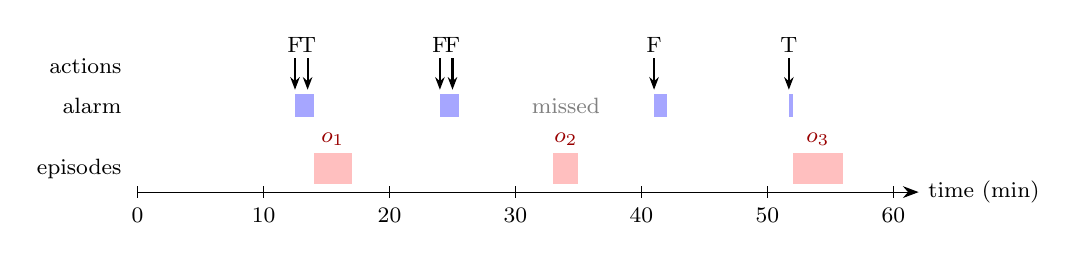
\begin{tikzpicture}[x=0.16cm,y=0.5cm,font=\footnotesize]
\draw[-{Stealth[length=2mm]}] (0,0) -- (62,0) node[right]{time (min)};
\foreach \x in {0,10,20,30,40,50,60} \draw (\x,0.15) -- (\x,-0.15) node[below]{\x};
\fill[red!25] (14,0.2) rectangle (17,1.0); \node[red!60!black] at (15.5,1.35) {$o_1$};
\fill[red!25] (33,0.2) rectangle (35,1.0); \node[red!60!black] at (34,1.35) {$o_2$};
\fill[red!25] (52,0.2) rectangle (56,1.0); \node[red!60!black] at (54,1.35) {$o_3$};
\node[anchor=east] at (-0.5,0.6) {episodes};
\fill[blue!35] (12.5,1.9) rectangle (14,2.5);
\fill[blue!35] (24,1.9) rectangle (25.5,2.5);
\fill[blue!35] (41,1.9) rectangle (42,2.5);
\fill[blue!35] (51.7,1.9) rectangle (52,2.5);
\node[anchor=east] at (-0.5,2.2) {alarm};
\foreach \x/\c in {12.5/F,13.5/T,24/F,25/F,41/F,51.7/T}
  {\draw[-{Stealth[length=1.6mm]},thick] (\x,3.4) -- (\x,2.6); \node at (\x,3.75) {\c};}
\node[anchor=east] at (-0.5,3.2) {actions};
\node[gray] at (34,2.2) {missed};
\end{tikzpicture}
\caption{Worked example (one link, one exposure hour, $H=60$\,s, a measurement every
2\,s). Red: degradation episodes with onsets $o_1,o_2,o_3$. Blue: alarm runs.
Arrows: actions, each valid for 60\,s, marked true (T) or false (F). The 90\,s run
before $o_1$ fires at 12.5\,min (window ends before $o_1$: false) and is renewed at
13.5\,min (true, lead 30\,s). $o_2$ is missed; the run before $o_3$ fires 18\,s
before it. $\DR_{60}=2/3$, $\FAR=4$ per hour, duty 7.2\%.}
\label{fig:example}
\end{figure}

Fig.~\ref{fig:example} shows the measures for one link and one hour at $H=60$\,s.
The alarm is on before $o_1$ and $o_3$, so $\DR_{60}=2/3$. Of six actions, two are
true and four false, so $\FAR=4$ per hour. Keeping the first alarm on for 90\,s cost
an extra (false) action and did not lengthen the lead beyond $H$: the earliest
action covering $o_1$ is the renewal 30\,s before it. Sample-level metrics tell a
different story. Of the 129 alarmed measurements, 39 are followed by an onset within
60\,s, so precision is 0.30; with 90 such measurements in the hour, recall is 0.43
and $F_1=0.36$. A second predictor that raises one 60\,s alarm before $o_1$ and five
isolated one-measurement alarms elsewhere has precision 0.86, recall 0.33 and
$F_1=0.48$, so sample metrics prefer it, yet it warns about one onset instead of two
and wastes five actions per hour instead of four.

%% ===================================================================
\section{Experimental design}
\label{sec:design}

\subsection{Datasets}
\label{sec:data}

\begin{table}[!htbp]
\centering
\caption{Datasets after preprocessing. Links with $\ge1$ onset in brackets;
exposure hours, warnable onsets and positive rates follow Section~\ref{sec:model}
(exposure and warnable onsets at $H=30$\,s).}
\label{tab:data}
\resizebox{\linewidth}{!}{%
\begin{tabular}{lccccccc}
\toprule
Dataset & Measurements & Links & Observed h & Exposure h & Onsets (warnable) & Degraded \% & Positive \%, $H=10/30/60$ \\
\midrule
Cork 5G NSA & 164,735 & 82 (67) & 50.7 & 48.4 & 528 (521) & 1.8 & 2.6 / 6.0 / 9.5 \\
Cork 4G & 117,707 & 133 (119) & 36.3 & 28.5 & 1,906 (1,833) & 19.0 & 14.9 / 30.8 / 44.4 \\
Manaus (exploratory) & 167,479 & 1,033 (169) & 184.5 & 104.8 & 1,248 (883) & 13.0 & 3.8 / 9.0 / 13.8 \\
\bottomrule
\end{tabular}}
\end{table}

All three datasets are public and record RSRP, RSRQ, SINR and CQI from Android
measurement applications (Table~\ref{tab:data}).

\emph{Cork 5G NSA} \cite{raca2020}: 83 sessions recorded with G-NetTrack Pro in
2019--2020 on one Irish operator's network, driving (60) or static (23), while
streaming video or downloading files, at one sample per second. The UE is mostly in
5G non-standalone mode, so the channel measurements refer to the LTE anchor.
\emph{Cork 4G} \cite{raca2018}: 135 sessions recorded in 2017--2018 on two operators'
LTE networks (101 and 34 sessions), labelled static (15), pedestrian (31), car (53),
bus (16) and train (20) in the released files, at one sample per second. In both
Cork datasets one trace file is one session of one device and is the link unit, and
measurements without CQI (2G or 3G) end a segment. These datasets are the primary
evidence.

\emph{Manaus} \cite{silva2024}: the Manaus file of the Amazonas multi-operator
dataset (August 2023--April 2024), 526{,}200 rows. It has no device identifier, so a
link is a device model on a serving LTE cell, and measurements of several phones of
one model on one cell can be interleaved; we keep one measurement per link and
second (167{,}479). Sampling is irregular (median about 2\,s). Because links are not
single-device trajectories, Manaus results are treated as exploratory.

The three datasets span degradation regimes from rare (Cork 5G NSA, 1.8\% of
measurements degraded, 10 onsets per hour) to frequent (Cork 4G, 19\%, 53 onsets
per hour). Thresholds, horizons and budgets are the same for all. One Cork 5G NSA
session and two Cork 4G sessions contain no measurement with both RSRP and CQI and
therefore yield no link, which is why Table~\ref{tab:data} lists 82 and 133 links.

\subsection{Predictors}
All predictors see only the eligible window of $W=20$ measurements.

\emph{Signal rules (no fitting).} \textbf{RSRP level}, $s=-\mathrm{RSRP}_t$;
\textbf{RSRP trend}, minus a least-squares extrapolation of the last ten RSRP values
to $t+H$; \textbf{RSRP smoothed}, minus an exponentially weighted average of the
window ($\alpha=0.3$); \textbf{RSRP+CQI margin},
$s=-\max(\mathrm{RSRP}_t-\theta_P,\;2\,\mathrm{dB}\times(\mathrm{CQI}_t-\theta_C))$, the
distance to the degradation region in both quantities; an \textbf{A2 rule}, modelled
on measurement event A2 (serving cell becomes worse than a threshold) used to trigger
measurement and handover procedures \cite{ts38331}: the alarm turns on when
$\mathrm{RSRP}+h<\theta$ for each of the last $k$ measurements (time-to-trigger) and off
when $\mathrm{RSRP}-h>\theta$, with $\theta$ calibrated like $\tau$ and $k=3$, $h=2$\,dB
(variants $k=1,5$ and $h=0$ are in the released results); and \textbf{Random}, an
uninformed score.

\emph{Learned predictors.} Logistic regression (LR, class-balanced, standardised)
on three input sets: current RSRP and CQI only (same input as the margin rule), the
eight RSRP window statistics (same input as the RSRP rules), and all 37 window
features (for each channel the last value, mean, standard deviation, minimum,
maximum, change over the window and over the last five samples and slope; mean
sampling gap; fractions below the RSRP and CQI thresholds; fractions of missing
RSRQ and SINR). LR has no early stopping and is fitted on the fitting and
early-stopping links together. \textbf{XGBoost} \cite{chen2016xgboost} (600 trees, depth 6, learning
rate 0.05, early stopping on AUPRC) uses the 37 features. An \textbf{LSTM}
\cite{hochreiter1997} (two layers of 64 units) and a \textbf{Transformer} encoder
\cite{vaswani2017} (width 64, two layers, four heads) read the raw window with
missing indicators and the log sampling gap, trained with class-weighted
cross-entropy, Adam and early stopping. The three nonlinear models use three seeds.
Hyperparameters are fixed in advance and identical for all datasets. We did not tune
them against the event-level objective, which would require links beyond the fitting,
early-stopping and calibration sets; the comparison therefore concerns model families
trained with a conventional loss and given an event-level threshold, and gains from
event-level tuning are not excluded.

\subsection{Protocol}
\label{sec:protocol}
Links are assigned to five outer folds. For outer fold $k$, the training links are
split, by link and with a recorded seed, into fitting (70\%), early-stopping (10\%)
and calibration (20\%) links. The model is fitted on the fitting links, with epochs
or trees selected on the early-stopping links, and then frozen; it scores the
calibration links and the test links of fold $k$. For each budget
$\beta\in\{0.25,0.5,1,2,3,5,8\}$ per hour the threshold maximising $\DR_H$ subject
to $\FAR\le\beta$ on the calibration links (all of 200 candidate quantiles and
$\tau=+\infty$, alarm off, are evaluated) is applied to the test links of fold $k$. Every link is tested once, by a model
and threshold that never used it. Score files carry the row identifiers, labels and
split manifest, and the evaluator verifies them against the rebuilt task.

\emph{Primary comparison: matched realised rate.} For each predictor and seed, the
seven test operating points form an empirical frontier of detection against
realised false-action rate; we take its upper envelope (an operator can always
alarm less) and interpolate linearly in $\log\FAR$ at 1, 2 and 4 false actions per
hour, averaging over the seeds whose operating points span the rate (support is
reported). This describes what an operator choosing among the calibrated operating
points can achieve, not a single frozen policy at exactly that rate. Uncertainty
comes from 2{,}000 paired bootstrap resamples of links: in each resample every
operating point of every predictor is recomputed from per-link counts on the same
links, the envelope and interpolation are redone, and the difference from RSRP level
is taken. Intervals are pointwise 95\% percentile intervals without adjustment for
the many comparisons, and we read them as descriptive: we say whether an interval
includes zero but do not call individual differences significant. Because the frontier
is built from test operating points, a matched-rate value interpolates between policies
that were each calibrated out of sample; it is not itself a policy calibrated to the
target rate, and it is optimistic to the extent that an operator could not choose among
operating points after observing their test outcomes. Taking the upper envelope changed
one of the 437 interpolated values (by 0.04).

\emph{Secondary comparison: fixed policies.} For seed~0 at a nominal budget of two
false actions per hour, 1{,}000 paired link resamples give intervals for detection,
realised rate and their differences from RSRP level. These policies generally
realise different false-action rates, so this comparison is not at equal cost.
Accuracy is pooled test AUROC and AUPRC. A sensitivity analysis at $H=30$\,s varies
the degradation definition ($\theta_P=-105$\,dBm; $\theta_C=5$; $m=3$) and the window
($W=10,40$) for RSRP level, the margin rule, LR and XGBoost.

\emph{Service-level event.} To test whether the results depend on an event defined by
the same radio quantities that the rules threshold, we repeat the evaluation with an
event defined only by delivered downlink throughput: a measurement is degraded if
throughput is below 1\,Mbit/s, an episode needs $m=3$ consecutive degraded measurements,
and onsets, eligibility and labels follow Section~\ref{sec:model}. Inputs are unchanged
(radio measurements only). We use the Cork 5G NSA file-download sessions, since
video sessions are paced by the application (20 sessions with usable measurements,
11.5 observed hours, 127 onsets), and all Cork 4G sessions, whose application is not
recorded (36.3 hours, 593 onsets). The rules, LR and XGBoost (three seeds) are
retrained and evaluated with the same protocol; the LSTM and Transformer are not. A
relative definition (throughput below half the median of the previous ten
measurements) marked ordinary fluctuations as events on the download sessions, with
103 onsets per hour and 65\% of moments positive at $H=30$\,s, and is not used.

\subsection{Pre-training checks}
\label{sec:checks}
On every dataset we verified, before training, that (i) perturbing measurements
after a point in time leaves all earlier features, imputations and eligibility
unchanged; (ii) the exclusion mask (an episode observably under way) at $t$ equals
``the last $m$ measurements up to $t$ are degraded'' exactly, eligibility further
requiring $W$ measurements of history; (iii) always-off gives $\DR=0$, $\FAR=0$;
always-on gives $\DR=1$ with 102--120 false actions per hour at $H=30$\,s; the oracle
gives $\DR=1$, $\FAR=0$; and every lead is at most $H$; (iv) at a segment boundary
(measurements at $t=0,\dots,45$\,s, $W=20$, $H=30$\,s, a degradation starting at
$t=44$\,s) the onset is warnable, and always-on and the oracle detect it with the
true action counted; and (v) the threshold search evaluates the complete candidate
grid, since the false-action rate is not monotone in the threshold (merging alarm
runs changes when actions renew); and (vi) an independent replay that scores every
eligible moment, censored ones included, fires and renews actions, and classifies them
only afterwards gives the same detection, false actions, duty and leads as the
evaluator, in 108 comparisons on synthetic traces with frequent segment ends. All checks passed; the logs are part of the
release. Appendix~\ref{app:history} records two defects of earlier evaluator versions
that these checks exposed.

%% ===================================================================
\section{Results}
\label{sec:results}

\subsection{Accuracy view}

\begin{table}[!htbp]
\centering
\caption{Pooled test AUPRC (mean over seeds). Bold: best non-random predictor in the
column.}
\label{tab:auprc}
\resizebox{\linewidth}{!}{%
\begin{tabular}{lccccccccc}
\toprule
 & \multicolumn{3}{c}{Cork 5G NSA} & \multicolumn{3}{c}{Cork 4G} & \multicolumn{3}{c}{Manaus (exploratory)}\\
\cmidrule(lr){2-4}\cmidrule(lr){5-7}\cmidrule(lr){8-10}
$H$ (s) & 10 & 30 & 60 & 10 & 30 & 60 & 10 & 30 & 60 \\
\midrule
Base rate & 0.026 & 0.060 & 0.095 & 0.149 & 0.308 & 0.444 & 0.038 & 0.090 & 0.138 \\ \midrule
Random (uninformed) & 0.026 & 0.060 & 0.096 & 0.147 & 0.307 & 0.444 & 0.039 & 0.090 & 0.140 \\
RSRP level & 0.166 & 0.254 & 0.289 & 0.306 & 0.522 & 0.644 & 0.088 & 0.206 & 0.312 \\
RSRP trend & 0.154 & 0.169 & 0.205 & 0.312 & 0.483 & 0.573 & 0.091 & 0.225 & 0.303 \\
RSRP smoothed & 0.168 & 0.260 & 0.296 & 0.304 & 0.521 & 0.644 & 0.088 & 0.206 & 0.316 \\
RSRP+CQI margin & 0.164 & 0.269 & 0.307 & 0.327 & 0.555 & 0.679 & 0.115 & 0.253 & 0.371 \\
LR, current RSRP+CQI & 0.236 & 0.352 & 0.369 & 0.324 & 0.542 & 0.659 & 0.111 & 0.246 & 0.350 \\
LR, RSRP window & 0.243 & 0.359 & 0.391 & 0.342 & 0.577 & 0.703 & 0.100 & 0.229 & 0.321 \\
LR, all features & \textbf{0.315} & 0.443 & 0.464 & 0.380 & 0.607 & 0.717 & 0.220 & \textbf{0.439} & \textbf{0.596} \\
XGBoost & 0.294 & \textbf{0.457} & \textbf{0.489} & \textbf{0.438} & \textbf{0.623} & \textbf{0.728} & 0.222 & 0.426 & 0.544 \\
LSTM & 0.261 & 0.416 & 0.456 & 0.345 & 0.578 & 0.693 & 0.208 & 0.391 & 0.477 \\
Transformer & 0.271 & 0.426 & 0.436 & 0.378 & 0.599 & 0.716 & \textbf{0.231} & 0.400 & 0.543 \\
\bottomrule
\end{tabular}}
\end{table}

By sample-level accuracy, learning helps everywhere (Table~\ref{tab:auprc}). The four
full-feature learned model families (LR on all features, XGBoost, the LSTM and the
Transformer) have higher AUPRC than every signal
rule at every horizon in every dataset, and generally higher AUROC (Table~\ref{tab:auroc}; learned
0.82--0.94 against 0.63--0.86 in Cork 5G NSA, 0.77--0.84 against 0.61--0.80 in Cork 4G,
0.84--0.91 against 0.69--0.80 in Manaus). Relative to RSRP level, their AUPRC is
1.5--1.9 times higher in Cork 5G NSA, 1.1--1.4 times in Cork 4G and 1.5--2.6 times in
Manaus.

\subsection{Operational view at a matched false-action rate}

\begin{figure}[!htbp]
\centering
\includegraphics[width=\linewidth]{fig2_dr_far.pdf}
\caption{Share of warnable onsets warned against the realised false-action rate on
unseen links, at the seven calibrated budgets. Lines: mean over seeds; markers:
individual operating points. Rows: datasets; columns: horizons.}
\label{fig:drfar}
\end{figure}

\begin{table}[!htbp]
\centering
\caption{Share of warnable onsets warned at a matched realised rate of two false
actions per hour (upper envelope of the test operating points, interpolated in
$\log\FAR$; mean over seeds). Bold: best non-random predictor in the column.
Superscripts: number of seeds whose operating points span this rate when fewer than
three; --: not spanned. Paired intervals for the differences from RSRP level are in
Fig.~\ref{fig:matched} and the released results.}
\label{tab:matched}
\resizebox{\linewidth}{!}{%
\begin{tabular}{lccccccccc}
\toprule
 & \multicolumn{3}{c}{Cork 5G NSA} & \multicolumn{3}{c}{Cork 4G} & \multicolumn{3}{c}{Manaus (exploratory)}\\
\cmidrule(lr){2-4}\cmidrule(lr){5-7}\cmidrule(lr){8-10}
$H$ (s) & 10 & 30 & 60 & 10 & 30 & 60 & 10 & 30 & 60 \\
\midrule
Random (uninformed) & 0.01 & 0.02 & 0.02 & 0.01 & 0.02 & 0.05 & 0.01 & 0.05 & 0.06 \\
RSRP level & 0.12 & \textbf{0.37} & 0.45 & 0.02 & 0.06 & 0.14 & 0.05 & 0.08 & 0.18 \\
RSRP trend & 0.10 & 0.09 & 0.14 & 0.03 & 0.09 & 0.16 & 0.05 & 0.16 & 0.27 \\
RSRP smoothed & 0.12 & 0.34 & 0.44 & 0.02 & 0.05 & 0.10 & 0.03 & 0.09 & 0.18 \\
RSRP+CQI margin & 0.06 & 0.24 & 0.45 & 0.01 & 0.06 & 0.17 & -- & 0.09 & 0.23 \\
LR, current RSRP+CQI & 0.09 & 0.26 & 0.44 & 0.02 & 0.06 & 0.09 & -- & 0.07 & 0.23 \\
LR, RSRP window & 0.11 & 0.22 & 0.33 & 0.03 & 0.09 & 0.21 & 0.04 & 0.11 & 0.24 \\
LR, all features & 0.11 & 0.30 & 0.41 & 0.02 & 0.08 & 0.24 & 0.08 & 0.25 & 0.38 \\
XGBoost & \textbf{0.13} & 0.33 & 0.50 & \textbf{0.04} & \textbf{0.12} & 0.20 & \textbf{0.15}$^{2}$ & \textbf{0.27} & \textbf{0.44} \\
LSTM & 0.09 & 0.34 & \textbf{0.51} & 0.02 & 0.08 & 0.20 & 0.15$^{2}$ & 0.20 & 0.37 \\
Transformer & 0.10 & 0.34 & 0.47 & 0.03 & 0.10 & \textbf{0.24}$^{2}$ & 0.11 & 0.21 & 0.41 \\
\bottomrule
\end{tabular}}
\end{table}

\begin{figure}[!htbp]
\centering
\includegraphics[width=\linewidth]{fig3_matched_diff.pdf}
\caption{Difference in the share of warnable onsets warned at a matched realised rate
of 1, 2 and 4 false actions per hour, each predictor minus RSRP level, with pointwise
95\% paired link-bootstrap intervals (2{,}000 resamples, interpolation repeated in
each resample). Missing markers: the rate is not spanned.}
\label{fig:matched}
\end{figure}

Fig.~\ref{fig:drfar}, Table~\ref{tab:matched} and Fig.~\ref{fig:matched} give the
operator's view. Whether learning warns about more degradations depends on the
dataset, the horizon and the rate, and is not predicted by the accuracy gains.

\emph{Cork 5G NSA.} At one and two false actions per hour no learned model warns about
more onsets than the RSRP threshold. At two per hour and $H=30$\,s it warns about 37\% of onsets
against 30--34\% for the learned models; the paired differences are $-0.07$
(interval $-0.14$ to $0.00$) for LR and $-0.03$ to $-0.04$, with intervals including
zero, for the nonlinear models. At one per hour and $H=60$\,s the interval for LR lies
below zero ($-0.14$, $-0.26$ to $-0.03$); with more than 100 pointwise intervals in
Fig.~\ref{fig:matched}, one interval excluding zero is weak evidence on its own. At two per hour and $H=60$\,s the LSTM and XGBoost warn about 51\% and 50\% against
45\% for RSRP level, but these differences ($+0.06$, $-0.04$ to $+0.14$; $+0.05$, $-0.05$
to $+0.12$) are uncertain and do not establish either superiority or equality. The
frontier view favours RSRP level partly because its policies overshoot: its seed-0
policy for two per hour realised 2.02 at $H=30$\,s and 2.58 at $H=60$\,s.
Table~\ref{tab:cap} instead takes, for each predictor, the best of its seven policies
whose realised rate stayed at or below two per hour. In that view RSRP level warns about
28\% of onsets at $H=30$\,s against 26--32\% for the learned models, and 44\% at
$H=60$\,s against 37--47\%. Both views select among test operating points and neither
is a frozen policy that met the cap by construction; together they show that on this
dataset the ranking of the threshold and the learned models is within a few points and
depends on how operating points are compared. Only at
the looser rate and longer horizon does an interval exclude zero in favour of a learned
model: at four per hour and $H=60$\,s the LSTM adds 15 points ($+0.02$ to $+0.23$) and
XGBoost 12 points ($-0.01$ to $+0.20$), despite
AUPRC gains of 1.5--1.9 times at every horizon.

\emph{Cork 4G.} Detection is low for every predictor (an onset about once a minute
makes two false actions per hour a strict budget), but learned models add a few
points. At two per hour and $H=30$\,s XGBoost warns about 12\% against 6\% for RSRP
level ($+0.06$, $+0.02$ to $+0.10$), and the Transformer and LSTM add 3--4 points with
lower interval limits at or just above zero. This gain rests on interpolation between
operating points: the seed-0 XGBoost policy calibrated to two per hour realised only
0.63 false actions per hour and warned about 6\% of onsets, whereas the RSRP level
policy realised 3.58 (Table~\ref{tab:paired}), so the matched value for XGBoost lies
between its policies for budgets of two and three (0.63 and 3.12 realised). The Cork 4G
advantage is therefore a property of the frontier, not of any single calibrated policy.
Within the cap (Table~\ref{tab:cap}) the learned models warn about 7\% against 4\% for
RSRP level and 5\% for the RSRP trend rule at $H=30$\,s; at $H=60$\,s LR warns about 24\% against 14\% ($+0.10$,
$0.00$ to $+0.19$). Here the RSRP trend rule and LR on the RSRP window alone also have
higher point estimates than RSRP level (intervals include zero), suggesting that part
of the gain comes from the recent history of the same signal.

\emph{Manaus (exploratory).} Learned models warn about substantially more onsets at
every rate where RSRP level can be compared: at two per hour, 12--18 points more at $H=30$\,s and 19--26 points
more at $H=60$\,s, with intervals excluding zero (XGBoost: 44\% against 18\% at
$H=60$\,s). Differences quoted in the text are computed from unrounded values and can
differ by one point from differences of the rounded entries in Table~\ref{tab:matched}.

\emph{Strict budgets.} At one false action per hour the best predictor warns about at
most 40\% of onsets in Cork 5G NSA (RSRP level, $H=60$\,s), 14\% in Cork 4G and 33\% in
Manaus (Table~\ref{tab:matchedall}, which gives all matched values at one, two and four
false actions per hour with their paired intervals). An operator who can afford one
wasted preventive action per hour of link time
should expect most degradations to go unwarned.

\emph{Same-input ablations.} LR on current RSRP and CQI stays within 0.08 of the margin
rule that uses the same inputs, in every dataset and horizon. LR on the RSRP window
is below RSRP level in Cork 5G NSA but above it in Cork 4G (Table~\ref{tab:matched}), so
the benefit of learning from the same signal is itself dataset-dependent.

\emph{Fixed policies.} Table~\ref{tab:paired} reports seed-0 policies calibrated to a
nominal two false actions per hour, with intervals for detection, realised rate and
their differences from RSRP level. Because these policies realise different rates (in
Cork 5G NSA at $H=30$\,s, 2.02 per hour for RSRP level against 1.36 for LR), they are not a
comparison at equal cost; they show what each calibrated policy actually delivered.
Table~\ref{tab:cap} gives the complementary within-cap view.

\begin{table}[!htbp]
\centering
\caption{Within-cap view: for each predictor and seed, the highest share of warnable
onsets warned among its seven test policies whose realised rate is at most two false
actions per hour (mean over seeds; realised false actions per hour in parentheses).
Superscripts: seeds with at least one policy within the cap, when fewer than three. The
choice among test operating points makes every entry optimistic.}
\label{tab:cap}
\resizebox{\linewidth}{!}{%
\begin{tabular}{lcccccc}
\toprule
 & \multicolumn{2}{c}{Cork 5G NSA} & \multicolumn{2}{c}{Cork 4G} & \multicolumn{2}{c}{Manaus (exploratory)}\\
\cmidrule(lr){2-3}\cmidrule(lr){4-5}\cmidrule(lr){6-7}
$H$ (s) & 30 & 60 & 30 & 60 & 30 & 60 \\
\midrule
RSRP level & 0.28 (1.24) & 0.44 (1.78) & 0.04 (1.09) & 0.07 (1.11) & 0.07 (1.72) & 0.17 (1.99) \\
RSRP trend & 0.06 (1.51) & 0.10 (1.51) & 0.05 (0.74) & 0.12 (1.28) & 0.10 (1.35) & 0.26 (1.87) \\
RSRP+CQI margin & 0.18 (1.40) & 0.39 (1.57) & 0.04 (1.44) & 0.17 (1.96) & 0.08 (1.56) & 0.16 (1.43) \\
A2 rule ($k=3$, $h=2$\,dB) & 0.29 (0.97) & 0.45 (1.20) & 0.02 (0.32) & 0.09 (1.18) & 0.07 (1.41) & 0.15 (1.65) \\
LR, all features & 0.29 (1.94) & 0.37 (1.68) & 0.07 (1.58) & 0.23 (1.89) & 0.24 (1.81) & 0.23 (1.23) \\
XGBoost & 0.26 (1.45) & 0.47 (1.67) & 0.07 (1.05) & 0.12 (1.06) & 0.19 (1.25) & 0.42 (1.66) \\
LSTM & 0.32 (1.85) & 0.46 (1.57) & 0.07 (1.51) & 0.14 (1.16) & 0.15 (1.38) & 0.32 (1.77) \\
Transformer & 0.30 (1.65) & 0.42 (1.45) & 0.07 (1.18) & 0.23$^{2}$ (1.84) & 0.18 (1.73) & 0.37 (1.66) \\
\bottomrule
\end{tabular}}
\end{table}

\begin{table}[!htbp]
\centering
\caption{Secondary comparison: fixed policies (seed~0, nominal budget two false
actions per hour) with 95\% paired link-bootstrap intervals. FAR: realised false
actions per exposure hour; DR: share of warnable onsets warned; $\Delta$DR:
difference from RSRP level on the same resampled links; Lead: median lead of detected
onsets (s). Realised rates differ between policies.}
\label{tab:paired}
\resizebox{\linewidth}{!}{%
\begin{tabular}{llcccc}
\toprule
Dataset, $H$ & Predictor & FAR [95\% CI] & DR [95\% CI] & $\Delta$DR vs RSRP level [95\% CI] & Lead \\
\midrule
\multirow{6}{*}{Cork 5G NSA, 30\,s} & RSRP level & 2.02 [1.20, 3.04] & 0.37 [0.29, 0.45] & -- & 18 \\
 & RSRP+CQI margin & 1.40 [0.93, 1.97] & 0.18 [0.12, 0.24] & -0.20 [-0.27, -0.13] & 17 \\
 & LR, all features & 1.36 [0.84, 2.03] & 0.23 [0.17, 0.29] & -0.14 [-0.21, -0.09] & 19 \\
 & XGBoost & 1.53 [0.94, 2.31] & 0.29 [0.21, 0.38] & -0.08 [-0.15, -0.03] & 21 \\
 & LSTM & 1.90 [1.11, 2.90] & 0.33 [0.24, 0.42] & -0.04 [-0.11, +0.02] & 19 \\
 & Transformer & 1.78 [1.22, 2.58] & 0.34 [0.27, 0.42] & -0.03 [-0.09, +0.02] & 19 \\
\midrule
\multirow{6}{*}{Cork 5G NSA, 60\,s} & RSRP level & 2.58 [1.17, 4.31] & 0.48 [0.39, 0.57] & -- & 41 \\
 & RSRP+CQI margin & 1.43 [1.00, 1.99] & 0.38 [0.32, 0.45] & -0.10 [-0.17, -0.03] & 36 \\
 & LR, all features & 1.68 [1.09, 2.41] & 0.37 [0.29, 0.44] & -0.11 [-0.18, -0.05] & 34 \\
 & XGBoost & 1.85 [1.21, 2.62] & 0.48 [0.39, 0.59] & +0.01 [-0.04, +0.05] & 44 \\
 & LSTM & 1.55 [1.04, 2.24] & 0.46 [0.37, 0.56] & -0.02 [-0.09, +0.05] & 41 \\
 & Transformer & 1.15 [0.75, 1.68] & 0.42 [0.33, 0.51] & -0.05 [-0.13, +0.01] & 37 \\
\midrule
\multirow{6}{*}{Cork 4G, 30\,s} & RSRP level & 3.58 [0.39, 8.31] & 0.07 [0.02, 0.14] & -- & 15 \\
 & RSRP+CQI margin & 1.44 [0.87, 2.12] & 0.04 [0.02, 0.05] & -0.04 [-0.11, +0.01] & 15 \\
 & LR, all features & 1.58 [0.93, 2.40] & 0.07 [0.05, 0.10] & -0.00 [-0.07, +0.05] & 14.5 \\
 & XGBoost & 0.63 [0.30, 1.06] & 0.06 [0.04, 0.08] & -0.02 [-0.09, +0.04] & 11.5 \\
 & LSTM & 3.12 [1.98, 4.51] & 0.13 [0.09, 0.17] & +0.06 [-0.03, +0.12] & 15 \\
 & Transformer & 1.58 [0.75, 2.71] & 0.07 [0.05, 0.09] & -0.00 [-0.08, +0.05] & 13 \\
\midrule
\multirow{6}{*}{Cork 4G, 60\,s} & RSRP level & 3.24 [1.31, 5.62] & 0.19 [0.13, 0.27] & -- & 34 \\
 & RSRP+CQI margin & 1.75 [1.13, 2.35] & 0.15 [0.12, 0.18] & -0.04 [-0.13, +0.03] & 33 \\
 & LR, all features & 1.89 [1.20, 2.66] & 0.23 [0.17, 0.28] & +0.04 [-0.05, +0.11] & 28 \\
 & XGBoost & 3.24 [1.54, 5.63] & 0.26 [0.22, 0.31] & +0.07 [-0.02, +0.15] & 29 \\
 & LSTM & 2.99 [1.49, 5.29] & 0.25 [0.20, 0.30] & +0.06 [-0.02, +0.14] & 30.5 \\
 & Transformer & 1.14 [0.59, 1.81] & 0.12 [0.09, 0.15] & -0.07 [-0.16, +0.00] & 27 \\
\midrule
\multirow{6}{*}{Manaus (exploratory), 30\,s} & RSRP level & 2.46 [0.93, 5.30] & 0.11 [0.02, 0.21] & -- & 15 \\
 & RSRP+CQI margin & 1.56 [0.68, 3.20] & 0.08 [0.02, 0.14] & -0.03 [-0.13, +0.06] & 21 \\
 & LR, all features & 1.81 [0.77, 4.05] & 0.24 [0.12, 0.37] & +0.13 [+0.04, +0.25] & 19 \\
 & XGBoost & 1.03 [0.34, 2.23] & 0.20 [0.09, 0.35] & +0.10 [-0.09, +0.29] & 19 \\
 & LSTM & 3.25 [1.08, 7.57] & 0.27 [0.11, 0.45] & +0.17 [-0.03, +0.36] & 16 \\
 & Transformer & 2.96 [0.69, 6.78] & 0.20 [0.08, 0.33] & +0.09 [-0.04, +0.26] & 18 \\
\midrule
\multirow{6}{*}{Manaus (exploratory), 60\,s} & RSRP level & 1.83 [0.79, 3.88] & 0.16 [0.06, 0.28] & -- & 31 \\
 & RSRP+CQI margin & 1.43 [0.64, 2.94] & 0.16 [0.08, 0.26] & +0.01 [-0.04, +0.06] & 36 \\
 & LR, all features & 2.03 [0.81, 4.14] & 0.38 [0.20, 0.55] & +0.23 [+0.11, +0.35] & 34 \\
 & XGBoost & 1.47 [0.58, 3.10] & 0.40 [0.21, 0.58] & +0.24 [+0.06, +0.44] & 35 \\
 & LSTM & 4.28 [1.53, 9.04] & 0.43 [0.23, 0.62] & +0.28 [+0.06, +0.49] & 36 \\
 & Transformer & 2.39 [1.09, 4.60] & 0.45 [0.26, 0.61] & +0.29 [+0.12, +0.46] & 37 \\
\bottomrule
\end{tabular}}
\end{table}

\subsection{Stronger received-power baselines}
\label{sec:strong}

\begin{table}[!htbp]
\centering
\caption{Share of warnable onsets warned at a matched realised rate of two false
actions per hour, with the paired difference from the A2 rule and its pointwise 95\%
link-bootstrap interval in parentheses (matched-rate protocol of
Table~\ref{tab:matched}). Superscripts: seeds spanning the rate when fewer than three.}
\label{tab:strong}
\resizebox{\linewidth}{!}{%
\begin{tabular}{lcccccc}
\toprule
 & \multicolumn{2}{c}{Cork 5G NSA} & \multicolumn{2}{c}{Cork 4G} & \multicolumn{2}{c}{Manaus (exploratory)}\\
\cmidrule(lr){2-3}\cmidrule(lr){4-5}\cmidrule(lr){6-7}
$H$ (s) & 30 & 60 & 30 & 60 & 30 & 60 \\
\midrule
RSRP level & 0.37 (-0.01 [-0.07, +0.02]) & 0.45 (-0.07 [-0.11, -0.01]) & 0.06 (0.00 [-0.04, +0.01]) & 0.14 (0.00 [-0.08, +0.05]) & 0.08 (-0.02 [-0.04, +0.01]) & 0.18 (+0.01 [-0.06, +0.08]) \\
RSRP trend & 0.09 (-0.29 [-0.38, -0.20]) & 0.14 (-0.38 [-0.50, -0.25]) & 0.09 (+0.03 [-0.02, +0.07]) & 0.16 (+0.03 [-0.07, +0.10]) & 0.16 (+0.05 [-0.02, +0.16]) & 0.27 (+0.10 [-0.01, +0.22]) \\
RSRP+CQI margin & 0.24 (-0.14 [-0.23, -0.06]) & 0.45 (-0.08 [-0.16, +0.02]) & 0.06 (0.00 [-0.06, +0.03]) & 0.17 (+0.04 [-0.07, +0.11]) & 0.09 (-0.01 [-0.10, +0.10]) & 0.23 (+0.06 [-0.04, +0.23]) \\
A2 rule ($k=3$, $h=2$\,dB) & 0.38 & 0.52 & 0.06 & 0.13 & 0.11 & 0.17 \\
LR, all features & 0.30 (-0.08 [-0.17, -0.01]) & 0.41 (-0.11 [-0.20, -0.02]) & 0.08 (+0.02 [-0.03, +0.05]) & 0.24 (+0.10 [-0.01, +0.18]) & 0.25 (+0.14 [+0.04, +0.29]) & 0.38 (+0.21 [+0.05, +0.40]) \\
XGBoost & 0.33 (-0.05 [-0.13, +0.03]) & 0.50 (-0.03 [-0.11, +0.05]) & 0.12 (+0.06 [+0.01, +0.09]) & 0.20 (+0.07 [0.00, +0.12]) & 0.27 (+0.16 [+0.07, +0.31]) & 0.44 (+0.27 [+0.13, +0.45]) \\
LSTM & 0.34 (-0.04 [-0.11, +0.04]) & 0.51 (-0.01 [-0.09, +0.07]) & 0.08 (+0.03 [-0.02, +0.05]) & 0.20 (+0.07 [0.00, +0.12]) & 0.20 (+0.09 [+0.01, +0.26]) & 0.37 (+0.20 [+0.06, +0.38]) \\
Transformer & 0.34 (-0.04 [-0.12, +0.03]) & 0.47 (-0.05 [-0.13, +0.03]) & 0.10 (+0.04 [-0.01, +0.06]) & 0.24$^{2}$ (+0.11 [-0.02, +0.18]) & 0.21 (+0.10 [+0.02, +0.28]) & 0.41 (+0.24 [+0.09, +0.42]) \\
\bottomrule
\end{tabular}}
\end{table}

The A2 rule, the received-power trigger that operators already configure for
measurement reporting, is the strongest simple baseline on Cork 5G NSA
(Table~\ref{tab:strong}). At two false actions per hour it warns about 38\% of onsets
at $H=30$\,s and 52\% at $H=60$\,s; every learned model is below it, by 1--11 points,
with intervals that include zero for XGBoost, the LSTM and the Transformer and lie below
zero for LR. At one false action per hour every learned model is below it as well, by
6--16 points; only at four per hour and
$H=60$\,s does the LSTM exceed it (by 9 points, interval 0.00 to 0.18). Its variants
($k=1,5$; $h=0$) warn about 33--38\% and 46--52\% of onsets. Within the cap
(Table~\ref{tab:cap}) it warns about 29\% and 45\%, against 26--32\% and 37--47\% for the
learned models. On Cork 4G the A2 rule performs like RSRP level, and the strongest
rules are the RSRP trend and the margin rule; against the trend rule, XGBoost adds 2 points at $H=30$\,s ($-0.01$ to $+0.06$),
and LR and the Transformer add 7--8 points at $H=60$\,s with lower interval limits at or
just below zero. In Manaus the learned models exceed every rule, by 9--27 points over
the A2 rule, with intervals excluding zero, and by 4--17 points over the trend rule,
with intervals excluding zero for most comparisons.

\subsection{Warning lead and alarm duty}
By construction a lead lies in $(0,H]$. The median lead of detected onsets at two
false actions per hour is 4--9\,s for $H=10$\,s, 12--21\,s for $H=30$\,s and
26--44\,s for $H=60$\,s (Table~\ref{tab:lead}), but the uninformed random policy has
similar conditional leads (2--5, 13--19 and 25--29\,s), so lead conditional on
detection mostly reflects $H$ and the renewal rule rather than predictive
information. Alarms are on for a small fraction of the time at these budgets (median
duty 0.2--2.1\% across datasets and horizons; duty counts time with the score above threshold, which can differ
from the time an issued action keeps resources reserved). For handover preparation or
a carrier switch, which typically complete well within a second \cite{tayyab2019}, the
binding constraint is how many degradations are warned, not how early.

\subsection{False-action budgets do not transfer reliably}
\label{sec:transfer}

\begin{figure}[!htbp]
\centering
\includegraphics[width=\linewidth]{fig5_budget.pdf}
\caption{Budget-transfer ratio $\rho$ (realised false-action rate on unseen links
divided by the budget) for every horizon, budget and seed; bars: medians. Ratios
below 0.05, including zero, are drawn at 0.05; the largest ratio is 15.1.}
\label{fig:rho}
\end{figure}

A threshold chosen on calibration links does not reliably deliver its budget on new
links (Fig.~\ref{fig:rho}). Pooled over predictors, budgets, horizons and seeds, the
median ratio is 0.94 (Cork 5G NSA), 1.14 (Cork 4G) and 1.07 (Manaus); the 90th
percentiles are 1.56, 2.12 and 3.12; and the maxima are 3.5, 14.8 and 15.1 (an LSTM,
a Transformer and an LSTM at the tightest budget of 0.25 per hour). Overshoot occurs
for the simple rules too: the smoothed RSRP rule has a median ratio of 1.90 in Cork 4G.
Ratios below one, typical of the random score (medians 0.52, 0.81 and 0.46) and the
margin rule (0.55, 0.71 and 0.77), mean the threshold is needlessly conservative on new
links and gives away detection. Because the largest ratios occur at the tightest budget,
where a few extra false actions inflate $\rho$, the absolute excess $\FAR-\beta$ is
also informative (the Cork 4G maximum of 14.8 times the budget is 3.71 false actions
per hour against a budget of 0.25): at $\beta=0.25$ it is at most 0.6, 3.5 and 3.5 false actions per hour
in the three datasets, and over all budgets at most 3.4, 7.2 and 14.5, in each case for
the smoothed RSRP rule; 43\%, 61\% and 55\% of operating points exceed their budget. We hypothesise that
the main causes are estimating an extreme threshold from a limited set of calibration
links (20\% of the training links) and heterogeneity between links; the present design
does not separate these from split-to-split variation, which a calibration-size
ablation would. Online recalibration per cell or link is a plausible remedy that we
have not evaluated.

\subsection{Accuracy and operational benefit}

\begin{figure}[!htbp]
\centering
\includegraphics[width=\linewidth]{fig4_auprc_vs_dr.pdf}
\caption{AUPRC (accuracy view) against detection at a matched two false actions per
hour (operational view) at $H=30$\,s; one marker per predictor and seed.}
\label{fig:auprc}
\end{figure}

Fig.~\ref{fig:auprc} sets the two views side by side. Within the learned models, AUPRC
and matched-rate detection are positively correlated in all nine dataset--horizon
settings (Kendall $\tau$ 0.24--0.70), but each value rests on 9--12 model--seed points
and only five of the nine would exclude zero at the 5\% level without adjustment, so
accuracy ranks learned models against each other only loosely. It does not predict whether, or by how much, they beat a simple
rule: Cork 5G NSA has AUPRC gains over RSRP level similar to Manaus (1.5--1.9 against
1.5--2.6 times) but no operational gain at strict rates, where the RSRP threshold, with
the lowest AUPRC of the main predictors, has the highest detection at $H=30$\,s;
Cork 4G has the smallest AUPRC gains and a small but detectable operational gain.

\subsection{Is the degradation proxy meaningful?}
\label{sec:proxy}
We compare delivered downlink throughput inside and outside episodes descriptively.
In Cork 5G NSA file-download sessions (21 sessions, 35{,}060 measurements with a
throughput value, 159 onsets), the median is 4.7\,Mbit/s inside episodes against
17.4\,Mbit/s outside, and 18\% against 11\% of measurements are below 1\,Mbit/s.
Video-streaming sessions are paced by the application and show no difference. The
Cork 4G files do not record the application, so all 117{,}707 measurements (1{,}906
onsets) are pooled: 2.3 against 11.3\,Mbit/s, and 33\% against 10\% below 1\,Mbit/s.
At the onset itself the change is gradual: the median ratio of throughput in the
10\,s after to the 10\,s before an onset is 0.95 (5G downloads) and 0.92 (4G), and
17--19\% of onsets are followed by a drop of more than half. The proxy marks periods
of poorer service rather than abrupt failures; these comparisons are descriptive and
not adjusted for location or load.

\subsection{Sensitivity}
\label{sec:sens}

\begin{table}[!htbp]
\centering
\caption{Sensitivity at $H=30$\,s (seed~0, nominal two false actions per hour):
DR (realised FAR) under alternative degradation definitions and window lengths.
Realised rates differ between entries, so rankings are indicative.}
\label{tab:sens}
\resizebox{\linewidth}{!}{%
\begin{tabular}{llcccccc}
\toprule
Dataset & Predictor & Main & RSRP $<-105$ & CQI $<5$ & $m=3$ & $W=10$ & $W=40$ \\
\midrule
\multirow{4}{*}{Cork 5G NSA} & RSRP level & 0.37 (2.0) & 0.46 (1.8) & 0.26 (2.0) & 0.34 (2.1) & 0.37 (2.0) & 0.37 (2.0) \\
 & RSRP+CQI margin & 0.18 (1.4) & 0.19 (1.0) & 0.12 (0.8) & 0.19 (1.6) & 0.18 (1.4) & 0.18 (1.4) \\
 & LR, all features & 0.23 (1.4) & 0.26 (1.5) & 0.13 (1.1) & 0.20 (1.3) & 0.17 (1.6) & 0.28 (1.9) \\
 & XGBoost & 0.29 (1.5) & 0.27 (1.6) & 0.17 (1.0) & 0.15 (0.8) & 0.36 (1.9) & 0.35 (2.1) \\
\midrule
\multirow{4}{*}{Cork 4G} & RSRP level & 0.07 (3.6) & 0.10 (3.4) & 0.06 (4.6) & 0.07 (2.7) & 0.11 (2.6) & 0.07 (3.6) \\
 & RSRP+CQI margin & 0.04 (1.4) & 0.06 (1.5) & 0.01 (0.2) & 0.01 (0.2) & 0.04 (1.4) & 0.04 (1.4) \\
 & LR, all features & 0.07 (1.6) & 0.10 (1.4) & 0.11 (2.7) & 0.06 (1.7) & 0.09 (1.9) & 0.06 (1.5) \\
 & XGBoost & 0.06 (0.6) & 0.12 (1.6) & 0.08 (1.6) & 0.09 (1.9) & 0.13 (2.3) & 0.06 (1.1) \\
\midrule
\multirow{4}{*}{Manaus (exploratory)} & RSRP level & 0.11 (2.5) & 0.09 (1.9) & 0.09 (1.2) & 0.08 (2.9) & 0.06 (2.4) & 0.12 (4.9) \\
 & RSRP+CQI margin & 0.08 (1.6) & 0.08 (1.1) & 0.05 (0.7) & 0.08 (3.4) & 0.09 (2.3) & 0.23 (5.2) \\
 & LR, all features & 0.24 (1.8) & 0.18 (1.7) & 0.14 (1.2) & 0.25 (2.0) & 0.25 (2.8) & 0.40 (3.8) \\
 & XGBoost & 0.20 (1.0) & 0.19 (0.9) & 0.17 (0.7) & 0.43 (3.0) & 0.43 (4.8) & 0.52 (5.8) \\
\bottomrule
\end{tabular}}
\end{table}

Table~\ref{tab:sens} shows that the qualitative picture at $H=30$\,s holds under the
alternative definitions and windows, with the caveat that these are nominal-budget
policies with unequal realised rates. In Cork 5G NSA, RSRP level warns about the most
onsets in all six variants, with XGBoost within 0.02 of it for $W=10$ and $W=40$. In
Cork 4G no predictor separates from the others. In Manaus, LR and XGBoost warn about more
onsets than RSRP level in every variant, by more with $W=40$ but at higher realised
rates.

\subsection{Service-level events}
\label{sec:tput}

\begin{table}[!htbp]
\centering
\caption{Throughput-defined event (downlink throughput below 1\,Mbit/s for at least
three measurements): share of warnable onsets warned at a matched realised rate of two
false actions per hour, with the paired difference from the A2 rule and its pointwise
95\% interval; --: not spanned. Lower block: pooled test AUROC / AUPRC and base rate.}
\label{tab:tput}
\resizebox{\linewidth}{!}{%
\begin{tabular}{lcccc}
\toprule
 & \multicolumn{2}{c}{Cork 5G NSA, downloads} & \multicolumn{2}{c}{Cork 4G}\\
\cmidrule(lr){2-3}\cmidrule(lr){4-5}
$H$ (s) & 30 & 60 & 30 & 60 \\
\midrule
RSRP level & 0.06 (+0.01 [-0.04, +0.04]) & 0.09 (+0.01 [-0.07, +0.06]) & 0.04 (+0.01 [0.00, +0.02]) & 0.06 (0.00 [-0.03, +0.03]) \\
RSRP trend & -- & 0.07 (-0.01 [-0.10, +0.06]) & 0.02 (-0.01 [-0.04, +0.01]) & 0.05 (-0.01 [-0.07, +0.03]) \\
RSRP+CQI margin & 0.03 (-0.02 [-0.07, +0.02]) & 0.08 (0.00 [-0.09, +0.05]) & 0.02 (-0.01 [-0.04, +0.02]) & 0.07 (+0.01 [-0.05, +0.06]) \\
A2 rule ($k=3$, $h=2$\,dB) & 0.05 & 0.08 & 0.03 & 0.06 \\
LR, all features & -- & -- & 0.06 (+0.03 [-0.01, +0.06]) & 0.11 (+0.05 [0.00, +0.10]) \\
XGBoost & 0.03 (-0.01 [-0.09, +0.02]) & 0.07 (-0.01 [-0.12, +0.06]) & 0.07 (+0.04 [0.00, +0.08]) & 0.10 (+0.04 [-0.02, +0.09]) \\
\midrule
\multicolumn{5}{l}{\emph{AUROC / AUPRC (base rate)}}\\
RSRP level & 0.48 / 0.10 & 0.45 / 0.15 & 0.60 / 0.15 & 0.58 / 0.24 \\
LR, all features & 0.60 / 0.12 & 0.59 / 0.20 & 0.72 / 0.23 & 0.70 / 0.33 \\
XGBoost & 0.55 / 0.10 & 0.58 / 0.20 & 0.71 / 0.23 & 0.70 / 0.34 \\
Base rate & 0.08 & 0.15 & 0.11 & 0.19 \\
\bottomrule
\end{tabular}}
\end{table}

With an event defined by delivered throughput (Table~\ref{tab:tput}), forecasting from
serving-cell radio measurements becomes much harder for every predictor. On the Cork 5G
NSA download sessions the received-power rules have AUROC below 0.5 and AUPRC close to
the base rate, the learned models reach AUROC 0.55--0.60, and at two false actions per hour
no predictor warns about more than 11\% of onsets, with no difference from the A2 rule
that excludes zero. On Cork 4G LR and XGBoost reach AUROC 0.70--0.72 against 0.58--0.60
for RSRP level and warn about 6--11\% of onsets, 3--5 points more than the A2 rule, with
lower interval limits at or just below zero. Most of the predictability of the main
event therefore comes from its definition in the same radio quantities that the inputs
measure; a drop in delivered throughput is only weakly anticipated by the serving
cell's radio measurements, whether by a rule or by a learned model. The comparison
between rules and learned models nonetheless points the same way as for the main
event: no gain on Cork 5G NSA and a small gain on Cork 4G.

%% ===================================================================
\section{Discussion}
\label{sec:discussion}

\paragraph{What the results mean for operators}
First, a degradation forecaster should be evaluated as a warning policy, by detection,
false actions per exposure hour, duty and lead at a stated budget, on links not used
for fitting or threshold selection, after checking that uninformed policies score as
they should. Second, standard received-power rules evaluated in exactly the same way
are essential baselines: on single-device 5G NSA traces no learned model warned about
more onsets than an A2-style rule at strict and moderate rates, although all full-feature
learned models were 1.5--1.9 times more accurate by AUPRC, and on 4G a rule using the
recent RSRP trend captured most of the learned models' gain. Third, an event defined in
the same radio quantities as the inputs is far easier to anticipate than a drop in
delivered service (Section~\ref{sec:tput}); claims about preventing service
degradation need a service-level event. Fourth, the benefit of learning, where it exists, appears at particular horizons
and rates, so it should be reported across the operating range rather than at a
single point. Fifth, budgets set offline should not be assumed to hold online.

\paragraph{Why might the datasets differ?}
Cork 5G NSA has rare degradations (1.8\% of measurements), Cork 4G frequent ones (19\%), and
Manaus links that are not single-device trajectories. In Manaus, interleaved
measurements of several devices make the current RSRP a noisier indicator, and window
statistics may carry information that a single-device trace does not need; Manaus also
has irregular sampling and many more links. In Cork 4G, frequent degradation makes the
recent trajectory of RSRP informative, which both the trend rule and the learned models
exploit. We cannot separate these explanations with the available data.

\paragraph{Threats to validity}
The main event is defined by RSRP and CQI thresholds and the strongest baselines
threshold RSRP, so part of their strength comes from closeness to the event definition.
The throughput-defined event (Section~\ref{sec:tput}) confirms that the main event is
easy to anticipate largely for this reason, and that a service-level event is hard for
every predictor; it rests on 127 onsets for Cork 5G NSA, so its intervals are wide, and a
throughput floor is itself only one service definition. With $m=2$ and $c=3$ at one sample per second, nearby episodes count separately,
and some of the 53 Cork 4G onsets per hour may be threshold chatter rather than distinct
events; a minimum gap between episodes would test this. The learned models use fixed
hyperparameters and a sample-level training loss (Section~\ref{sec:design}). The
bootstrap resamples links as independent units, although Cork sessions repeat routes and
Manaus links of one device model share devices across cells; folds and resamples grouped
by route or device model would be more conservative, and this dependence is one more
reason the Manaus result is treated as exploratory.

\paragraph{Limitations}
The degradation definition is a radio-quality proxy that tracks lower throughput but is
not a service or protocol failure. Calibration used 20\% of training links. Matched-rate
comparisons interpolate along an empirical frontier of seven operating points, and their
intervals are pointwise and unadjusted for multiplicity. Fixed-policy intervals do not
include refitting or recalibration variability, which the seed ranges partly show. The
models use only the serving cell's measurements; neighbour-cell measurements, the
natural additional input for handover, can be evaluated with the same protocol. The evaluation is offline: the benefit
of an action that is taken is assumed rather than measured.

%% ===================================================================
\section{Conclusion}
\label{sec:conclusion}
We specified radio degradation warning as preventive actions, each valid for a horizon
and charged when issued or renewed, and evaluated forecasters offline by detection and
false actions per exposure hour on links used neither for fitting nor for threshold
selection, after checking the specification against uninformed policies. Learned
forecasters were more accurate than received-power rules by AUPRC in every setting, but
at strict and moderate false-action rates none warned about more onsets than an
A2-style rule on single-device 5G NSA traces, and on 4G they added a few points; larger
gains appeared only on the exploratory multi-device Manaus data. With a throughput-defined
event, every predictor using serving-cell radio measurements warned about few onsets. Strict budgets left most
degradations unwarned, and thresholds set on calibration links could miss their budget
on new links by a large factor. Forecasting studies for network control should report
detection, realised false-action rate, duty and lead across a range of budgets, with
thresholds set out of sample, standard received-power rules evaluated in the same way,
and an event defined by the service the action is meant to protect.

%% ===================================================================
\section*{CRediT authorship contribution statement}
\textbf{David Olutunde Daniel}: Conceptualization, Methodology, Software, Formal
analysis, Investigation, Data curation, Visualization, Writing -- original draft,
Writing -- review \& editing.

\section*{Declaration of competing interest}
The author declares that he has no known competing financial interests or personal
relationships that could have appeared to influence the work reported in this paper.

\section*{Funding}
This work was conducted during a research internship at AT\&T, funded through Tech
Mahindra (Americas) Inc. Computations were performed on the Juno high-performance
computing cluster of The University of Texas at Dallas.

\section*{Data and code availability}
All datasets are public \cite{silva2024,raca2018,raca2020}; SHA-256 hashes of the
raw files used are given in the release. The release contains the preparation,
training and evaluation code, the pre-training check logs, the split manifests of all
213 training runs (1{,}065 outer-fold partitions), per-link evaluation counts from
which every operating point and bootstrap interval can be recomputed, and the software
environment; the scripts and outputs of the A2-rule and throughput-event analyses
(Sections~\ref{sec:strong} and \ref{sec:tput}) are included. It is available at
\url{https://github.com/david6070/radio-warning-evaluation} (release v1.0).

\section*{Declaration of generative AI and AI-assisted technologies in the writing process}
During the preparation of this work the author used a generative AI assistant for
help with editing text and code. After using this tool, the author reviewed and
edited the content as needed and takes full responsibility for the content of the
publication.


%% ===================================================================
\appendix
\section{Supplementary tables}
\label{app:tables}

\begin{table}[!htbp]
\centering
\caption{Pooled test AUROC (mean over seeds).}
\label{tab:auroc}
\resizebox{\linewidth}{!}{%
\begin{tabular}{lccccccccc}
\toprule
 & \multicolumn{3}{c}{Cork 5G NSA} & \multicolumn{3}{c}{Cork 4G} & \multicolumn{3}{c}{Manaus (exploratory)}\\
\cmidrule(lr){2-4}\cmidrule(lr){5-7}\cmidrule(lr){8-10}
$H$ (s) & 10 & 30 & 60 & 10 & 30 & 60 & 10 & 30 & 60 \\
\midrule
Random (uninformed) & 0.496 & 0.497 & 0.502 & 0.501 & 0.498 & 0.499 & 0.511 & 0.497 & 0.505 \\
RSRP level & 0.830 & 0.779 & 0.719 & 0.784 & 0.765 & 0.737 & 0.776 & 0.783 & 0.787 \\
RSRP trend & 0.801 & 0.690 & 0.632 & 0.752 & 0.673 & 0.609 & 0.760 & 0.725 & 0.688 \\
RSRP smoothed & 0.829 & 0.778 & 0.716 & 0.783 & 0.763 & 0.737 & 0.778 & 0.786 & 0.790 \\
RSRP+CQI margin & 0.865 & 0.810 & 0.747 & 0.795 & 0.777 & 0.751 & 0.799 & 0.800 & 0.805 \\
LR, current RSRP+CQI & 0.893 & 0.828 & 0.754 & 0.800 & 0.776 & 0.745 & 0.821 & 0.809 & 0.808 \\
LR, RSRP window & 0.916 & 0.883 & 0.843 & 0.803 & 0.792 & 0.775 & 0.796 & 0.797 & 0.797 \\
LR, all features & 0.938 & 0.901 & 0.858 & 0.825 & 0.805 & 0.780 & 0.905 & 0.903 & 0.913 \\
XGBoost & 0.917 & 0.882 & 0.857 & 0.845 & 0.816 & 0.794 & 0.878 & 0.871 & 0.870 \\
LSTM & 0.903 & 0.862 & 0.815 & 0.813 & 0.792 & 0.768 & 0.867 & 0.865 & 0.836 \\
Transformer & 0.913 & 0.876 & 0.822 & 0.826 & 0.803 & 0.782 & 0.891 & 0.882 & 0.873 \\
\bottomrule
\end{tabular}}
\end{table}

\begin{table}[!htbp]
\centering
\caption{Share of warnable onsets warned at a matched realised rate of one, two and four
false actions per hour (upper envelope of the test operating points, interpolated in
$\log\FAR$; mean over seeds), with the paired difference from RSRP level and its pointwise
95\% link-bootstrap interval in parentheses; Cork 5G NSA. Superscripts: number of seeds
spanning the rate when fewer than three; --: not spanned (no difference when RSRP level
does not span the rate).}
\label{tab:matchedall}
\resizebox{\linewidth}{!}{%
\begin{tabular}{llccc}
\toprule
$H$ & Predictor & 1 per hour & 2 per hour & 4 per hour \\
\midrule
\multirow{7}{*}{10\,s} & RSRP level & 0.06 & 0.12 & 0.20 \\
 & RSRP trend & 0.04 (-0.02 [-0.07, +0.01]) & 0.10 (-0.02 [-0.05, +0.02]) & 0.18 (-0.02 [-0.07, +0.03]) \\
 & RSRP+CQI margin & 0.03 (-0.03 [-0.08, -0.01]) & 0.06 (-0.06 [-0.10, -0.02]) & -- \\
 & LR, all features & 0.07 (+0.01 [-0.04, +0.03]) & 0.11 (-0.01 [-0.05, +0.03]) & 0.21 (+0.01 [-0.04, +0.06]) \\
 & XGBoost & 0.06 (0.00 [-0.05, +0.03]) & 0.13 (+0.01 [-0.03, +0.05]) & 0.23 (+0.03 [-0.02, +0.09]) \\
 & LSTM & 0.04 (-0.02 [-0.07, 0.00]) & 0.09 (-0.03 [-0.06, +0.02]) & 0.19 (-0.01 [-0.05, +0.03]) \\
 & Transformer & 0.05 (-0.01 [-0.05, +0.01]) & 0.10 (-0.02 [-0.05, +0.02]) & 0.20 (0.00 [-0.04, +0.04]) \\
\midrule
\multirow{7}{*}{30\,s} & RSRP level & 0.26 & 0.37 & 0.43 \\
 & RSRP trend & 0.04 (-0.21 [-0.31, -0.12]) & 0.09 (-0.28 [-0.36, -0.19]) & 0.18 (-0.24 [-0.37, -0.15]) \\
 & RSRP+CQI margin & 0.15 (-0.11 [-0.19, -0.04]) & 0.24 (-0.13 [-0.20, -0.05]) & 0.39 (-0.04 [-0.15, +0.04]) \\
 & LR, all features & 0.20 (-0.05 [-0.14, +0.03]) & 0.30 (-0.07 [-0.14, 0.00]) & 0.41 (-0.01 [-0.10, +0.07]) \\
 & XGBoost & 0.23 (-0.03 [-0.11, +0.05]) & 0.33 (-0.04 [-0.10, +0.04]) & 0.51 (+0.08 [-0.03, +0.17]) \\
 & LSTM & 0.20 (-0.05 [-0.12, +0.01]) & 0.34 (-0.03 [-0.08, +0.04]) & 0.49 (+0.07 [-0.03, +0.14]) \\
 & Transformer & 0.22 (-0.03 [-0.11, +0.04]) & 0.34 (-0.03 [-0.10, +0.04]) & 0.49 (+0.06 [-0.06, +0.13]) \\
\midrule
\multirow{7}{*}{60\,s} & RSRP level & 0.40 & 0.45 & 0.51 \\
 & RSRP trend & 0.07 (-0.33 [-0.44, -0.24]) & 0.14 (-0.30 [-0.44, -0.19]) & 0.25 (-0.27 [-0.46, -0.15]) \\
 & RSRP+CQI margin & 0.32 (-0.08 [-0.17, 0.00]) & 0.45 (0.00 [-0.11, +0.09]) & 0.63 (+0.11 [-0.03, +0.19]) \\
 & LR, all features & 0.27 (-0.14 [-0.26, -0.03]) & 0.41 (-0.04 [-0.15, +0.06]) & 0.55 (+0.04 [-0.10, +0.12]) \\
 & XGBoost & 0.33 (-0.07 [-0.14, +0.03]) & 0.50 (+0.05 [-0.05, +0.12]) & 0.64 (+0.12 [-0.01, +0.20]) \\
 & LSTM & 0.36 (-0.04 [-0.11, +0.04]) & 0.51 (+0.06 [-0.04, +0.14]) & 0.67 (+0.15 [+0.02, +0.23]) \\
 & Transformer & 0.35 (-0.05 [-0.14, +0.02]) & 0.47 (+0.02 [-0.07, +0.09]) & 0.60 (+0.09 [-0.03, +0.15]) \\
\bottomrule
\end{tabular}}
\end{table}

\begin{table}[!htbp]
\centering
\caption{As Table~\ref{tab:matchedall}, Cork 4G.}
\resizebox{\linewidth}{!}{%
\begin{tabular}{llccc}
\toprule
$H$ & Predictor & 1 per hour & 2 per hour & 4 per hour \\
\midrule
\multirow{7}{*}{10\,s} & RSRP level & 0.01 & 0.02 & 0.03 \\
 & RSRP trend & 0.02 (+0.01 [0.00, +0.01]) & 0.03 (+0.01 [0.00, +0.03]) & 0.06 (+0.03 [+0.02, +0.05]) \\
 & RSRP+CQI margin & 0.01 (-0.01 [-0.02, 0.00]) & 0.01 (-0.01 [-0.03, 0.00]) & 0.02 (-0.01 [-0.03, 0.00]) \\
 & LR, all features & -- & 0.02 (0.00 [-0.01, +0.01]) & 0.05 (+0.02 [-0.01, +0.03]) \\
 & XGBoost & 0.02 (+0.01 [0.00, +0.02]) & 0.04 (+0.02 [0.00, +0.03]) & 0.07 (+0.05 [+0.02, +0.07]) \\
 & LSTM & 0.01 (0.00 [-0.01, +0.01]) & 0.02 (0.00 [-0.01, +0.01]) & 0.04 (+0.01 [-0.01, +0.02]) \\
 & Transformer & 0.01 (0.00 [-0.01, +0.01]) & 0.03 (+0.01 [-0.01, +0.02]) & 0.05 (+0.02 [0.00, +0.04]) \\
\midrule
\multirow{7}{*}{30\,s} & RSRP level & 0.04 & 0.06 & 0.08 \\
 & RSRP trend & 0.06 (+0.02 [-0.01, +0.04]) & 0.09 (+0.04 [0.00, +0.07]) & 0.16 (+0.08 [-0.01, +0.11]) \\
 & RSRP+CQI margin & 0.03 (-0.01 [-0.04, +0.01]) & 0.06 (0.00 [-0.04, +0.03]) & 0.10 (+0.02 [-0.07, +0.04]) \\
 & LR, all features & 0.05 (+0.01 [-0.02, +0.04]) & 0.08 (+0.02 [-0.01, +0.06]) & 0.15 (+0.07 [-0.02, +0.11]) \\
 & XGBoost & 0.07 (+0.03 [0.00, +0.06]) & 0.12 (+0.06 [+0.02, +0.10]) & 0.19 (+0.11 [+0.04, +0.15]) \\
 & LSTM & 0.07$^{2}$ (+0.03 [0.00, +0.05]) & 0.08 (+0.03 [0.00, +0.06]) & 0.13 (+0.05 [0.00, +0.10]) \\
 & Transformer & 0.06 (+0.02 [0.00, +0.04]) & 0.10 (+0.04 [+0.01, +0.07]) & 0.16 (+0.08 [0.00, +0.11]) \\
\midrule
\multirow{7}{*}{60\,s} & RSRP level & 0.06 & 0.14 & 0.27 \\
 & RSRP trend & 0.11 (+0.04 [-0.02, +0.06]) & 0.16 (+0.03 [-0.07, +0.11]) & 0.31 (+0.04 [-0.08, +0.17]) \\
 & RSRP+CQI margin & 0.08 (+0.02 [-0.05, +0.05]) & 0.17 (+0.03 [-0.06, +0.12]) & 0.30 (+0.03 [-0.09, +0.17]) \\
 & LR, all features & 0.13 (+0.06 [-0.01, +0.12]) & 0.24 (+0.10 [0.00, +0.19]) & 0.35 (+0.08 [-0.03, +0.22]) \\
 & XGBoost & 0.12 (+0.06 [+0.01, +0.11]) & 0.20 (+0.06 [0.00, +0.16]) & 0.34 (+0.07 [0.00, +0.17]) \\
 & LSTM & 0.14 (+0.07 [+0.01, +0.12]) & 0.20 (+0.07 [0.00, +0.16]) & 0.34 (+0.07 [-0.01, +0.16]) \\
 & Transformer & 0.12$^{2}$ (+0.05 [-0.01, +0.12]) & 0.24$^{2}$ (+0.11 [-0.01, +0.19]) & 0.32 (+0.05 [-0.03, +0.23]) \\
\bottomrule
\end{tabular}}
\end{table}

\begin{table}[!htbp]
\centering
\caption{As Table~\ref{tab:matchedall}, Manaus (exploratory).}
\resizebox{\linewidth}{!}{%
\begin{tabular}{llccc}
\toprule
$H$ & Predictor & 1 per hour & 2 per hour & 4 per hour \\
\midrule
\multirow{7}{*}{10\,s} & RSRP level & 0.03 & 0.05 & 0.06 \\
 & RSRP trend & 0.04 (+0.01 [0.00, +0.02]) & 0.05 (+0.01 [0.00, +0.02]) & 0.07 (+0.01 [0.00, +0.03]) \\
 & RSRP+CQI margin & -- & -- & 0.02 (-0.04 [-0.11, +0.02]) \\
 & LR, all features & 0.05 (+0.02 [0.00, +0.08]) & 0.08 (+0.03 [+0.01, +0.16]) & 0.19 (+0.13 [+0.02, +0.28]) \\
 & XGBoost & 0.09$^{2}$ (+0.06 [+0.03, +0.12]) & 0.15$^{2}$ (+0.11 [+0.05, +0.19]) & 0.22 (+0.16 [+0.08, +0.29]) \\
 & LSTM & 0.09$^{2}$ (+0.05 [+0.02, +0.14]) & 0.15$^{2}$ (+0.10 [+0.03, +0.20]) & 0.20 (+0.14 [+0.05, +0.28]) \\
 & Transformer & 0.08$^{1}$ (+0.05 [+0.02, +0.12]) & 0.11 (+0.07 [+0.02, +0.18]) & 0.19 (+0.14 [+0.04, +0.28]) \\
\midrule
\multirow{7}{*}{30\,s} & RSRP level & -- & 0.08 & 0.13 \\
 & RSRP trend & 0.09 (--) & 0.16 (+0.07 [+0.01, +0.16]) & 0.25 (+0.12 [+0.02, +0.21]) \\
 & RSRP+CQI margin & 0.05 (--) & 0.09 (+0.01 [-0.07, +0.10]) & 0.14 (+0.01 [-0.09, +0.16]) \\
 & LR, all features & 0.11 (--) & 0.25 (+0.17 [+0.06, +0.29]) & 0.36 (+0.23 [+0.11, +0.39]) \\
 & XGBoost & 0.19$^{2}$ (--) & 0.27 (+0.18 [+0.10, +0.31]) & 0.39 (+0.26 [+0.13, +0.40]) \\
 & LSTM & 0.12 (--) & 0.20 (+0.12 [+0.04, +0.26]) & 0.36 (+0.23 [+0.08, +0.37]) \\
 & Transformer & 0.13 (--) & 0.21 (+0.13 [+0.04, +0.27]) & 0.34 (+0.21 [+0.08, +0.38]) \\
\midrule
\multirow{7}{*}{60\,s} & RSRP level & 0.05 & 0.18 & 0.31 \\
 & RSRP trend & 0.17 (+0.13 [+0.01, +0.20]) & 0.27 (+0.09 [-0.01, +0.23]) & 0.36 (+0.05 [-0.05, +0.20]) \\
 & RSRP+CQI margin & 0.12 (+0.08 [-0.02, +0.14]) & 0.23 (+0.05 [-0.04, +0.21]) & 0.40 (+0.08 [-0.05, +0.28]) \\
 & LR, all features & 0.20 (+0.15 [+0.05, +0.31]) & 0.38 (+0.20 [+0.06, +0.37]) & 0.59 (+0.27 [+0.10, +0.44]) \\
 & XGBoost & 0.33 (+0.28 [+0.14, +0.40]) & 0.44 (+0.26 [+0.13, +0.44]) & 0.57 (+0.25 [+0.11, +0.43]) \\
 & LSTM & 0.24$^{2}$ (+0.20 [+0.09, +0.34]) & 0.37 (+0.19 [+0.06, +0.37]) & 0.49 (+0.18 [+0.02, +0.37]) \\
 & Transformer & 0.28 (+0.23 [+0.09, +0.36]) & 0.41 (+0.23 [+0.10, +0.40]) & 0.58$^{2}$ (+0.27 [+0.10, +0.44]) \\
\bottomrule
\end{tabular}}
\end{table}

\begin{table}[!htbp]
\centering
\caption{Fixed policies (seed~0, nominal budget two false actions per hour): median lead of detected onsets (s) / alarm duty (\% of exposure time).}
\label{tab:lead}
\resizebox{\linewidth}{!}{%
\begin{tabular}{lccccccccc}
\toprule
 & \multicolumn{3}{c}{Cork 5G NSA} & \multicolumn{3}{c}{Cork 4G} & \multicolumn{3}{c}{Manaus (exploratory)}\\
\cmidrule(lr){2-4}\cmidrule(lr){5-7}\cmidrule(lr){8-10}
$H$ (s) & 10 & 30 & 60 & 10 & 30 & 60 & 10 & 30 & 60 \\
\midrule
Random (uninformed) & 5 / 0.0 & 18.5 / 0.0 & 28.5 / 0.0 & 3.5 / 0.0 & 18 / 0.1 & 27 / 0.1 & 2 / 0.0 & 13 / 0.1 & 25.5 / 0.1 \\
RSRP level & 5 / 0.3 & 18 / 0.8 & 41 / 1.3 & 7 / 0.6 & 15 / 1.9 & 34 / 5.4 & 7 / 1.3 & 15 / 1.8 & 31 / 2.8 \\
RSRP trend & 4 / 0.2 & 12 / 0.2 & 32 / 0.2 & 5 / 0.4 & 13 / 0.5 & 26 / 0.7 & 6 / 1.3 & 16.5 / 0.8 & 31 / 0.8 \\
RSRP smoothed & 5 / 0.5 & 18 / 1.4 & 40 / 2.4 & 6 / 2.5 & 16 / 2.5 & 34 / 5.8 & 6 / 1.6 & 15 / 2.4 & 34.5 / 3.2 \\
RSRP+CQI margin & 6.5 / 0.0 & 17 / 0.1 & 36 / 0.1 & 8 / 0.1 & 15 / 0.1 & 33 / 0.3 & 9 / 0.4 & 21 / 0.2 & 36 / 0.3 \\
LR, current RSRP+CQI & 6 / 0.2 & 19 / 0.3 & 39 / 0.3 & 7 / 0.2 & 18 / 0.2 & 36 / 4.5 & 9 / 0.4 & 19 / 1.1 & 38 / 1.3 \\
LR, RSRP window & 7 / 0.3 & 15 / 0.4 & 26.5 / 0.7 & 5 / 0.5 & 14 / 0.9 & 29 / 1.9 & 5 / 0.7 & 16 / 1.7 & 31 / 1.4 \\
LR, all features & 6 / 0.2 & 19 / 0.3 & 34 / 0.6 & 7 / 0.4 & 14.5 / 0.5 & 28 / 1.4 & 6 / 0.6 & 19 / 1.1 & 34 / 2.2 \\
XGBoost & 6 / 0.1 & 21 / 0.8 & 44 / 1.5 & 5 / 0.1 & 11.5 / 0.3 & 29 / 2.1 & 6 / 2.6 & 19 / 0.7 & 35 / 2.0 \\
LSTM & 4 / 0.3 & 19 / 1.0 & 41 / 1.5 & 5.5 / 0.3 & 15 / 1.3 & 30.5 / 3.2 & 6 / 2.5 & 16 / 2.5 & 36 / 5.7 \\
Transformer & 6 / 0.4 & 19 / 0.9 & 37 / 1.1 & 5 / 0.4 & 13 / 0.6 & 27 / 0.8 & 6 / 2.4 & 18 / 2.1 & 37 / 3.1 \\
\bottomrule
\end{tabular}}
\end{table}

\section{Defects found in earlier evaluator versions}
\label{app:history}
An earlier version of the evaluator renewed actions only at measurement times and failed
check (iii) of Section~\ref{sec:checks} on the irregularly sampled Manaus data
($\DR=0.89$ for always-on); the specification in Section~\ref{sec:measures} renews at the
expiry time itself. An earlier version of the threshold search stopped scanning after a
run of over-budget candidates; re-evaluating the saved predictions with the complete
grid changed none of the 1{,}071 operating points.

\newpage
%% ===================================================================
\begin{thebibliography}{99}

\bibitem{tayyab2019}
M.~Tayyab, X.~Gelabert, R.~J\"antti, A survey on handover management: from LTE to
NR, IEEE Access 7 (2019) 118907--118930. doi:10.1109/ACCESS.2019.2937301.

\bibitem{mollel2021survey}
M.~S. Mollel, A.~I. Abubakar, M.~Ozturk, S.~F. Kaijage, M.~Kisangiri, S.~Hussain,
M.~A. Imran, Q.~H. Abbasi, A survey of machine learning applications to handover
management in 5G and beyond, IEEE Access 9 (2021) 45770--45802.
doi:10.1109/ACCESS.2021.3067503.

\bibitem{alraih2023}
S.~Alraih, R.~Nordin, A.~Abu-Samah, I.~Shayea, N.~F. Abdullah, A survey on handover
optimization in beyond 5G mobile networks: challenges and solutions, IEEE Access 11
(2023) 59317--59345. doi:10.1109/ACCESS.2023.3284053.

\bibitem{polese2023}
M.~Polese, L.~Bonati, S.~D'Oro, S.~Basagni, T.~Melodia, Understanding O-RAN:
architecture, interfaces, algorithms, security, and research challenges, IEEE
Communications Surveys \& Tutorials 25~(2) (2023) 1376--1411.

\bibitem{pjanic2024}
D.~Pjanic, A.~Sopasakis, A.~Reial, F.~Tufvesson, Early-scheduled handover
preparation in 5G NR millimeter-wave systems, IEEE Open Journal of the
Communications Society 5 (2024) 6959--6971. doi:10.1109/OJCOMS.2024.3488594.

\bibitem{mollel2021}
M.~S. Mollel, M.~Abualhoul, G.~Simatwo, J.~Thompson, M.~Assimonis, Prediction of
coverage and quality of service in a real LTE network using deep learning, in:
Proc.\ IEEE PIMRC, 2021, pp.~1--6.

\bibitem{fauzi2022}
M.~F. Ahmad Fauzi, R.~Nordin, N.~F. Abdullah, H.~A.~H. Alobaidy, Mobile network
coverage prediction based on supervised machine learning algorithms, IEEE Access 10
(2022) 55782--55793. doi:10.1109/ACCESS.2022.3176619.

\bibitem{mohammadjafari2020}
S.~Mohammadjafari, S.~Roginsky, E.~Kavurmacioglu, M.~Cevik, J.~Ethier, A.~B. Bener,
Machine learning-based radio coverage prediction in urban environments, IEEE
Transactions on Network and Service Management 17~(4) (2020) 2117--2130.

\bibitem{lima2023}
J.~P. Lima, \'A.~A. de~Medeiros, E.~P. de~Aguiar, E.~F. Silva, V.~A. de~Sousa,
M.~L. Nunes, A.~L. Reis, Deep learning-based handover prediction for 5G and beyond
networks, in: Proc.\ IEEE ICC, 2023, pp.~3468--3473.
doi:10.1109/ICC45041.2023.10279195.

\bibitem{manalastas2023}
M.~Manalastas, M.~U.~B. Farooq, S.~M.~A. Zaidi, A.~Ijaz, W.~Raza, A.~Imran, Machine
learning-based handover failure prediction model for handover success rate
improvement in 5G, in: Proc.\ IEEE CCNC, 2023, pp.~684--685.
doi:10.1109/CCNC51644.2023.10059928.

\bibitem{chou2025}
P.-H. Chou, D.-C. Lin, H.-Y. Wei, W.~Saad, Y.~Tsao, Measurement-driven early warning
for resilient 5G NSA railway networks, arXiv:2511.08851v7, 2025.

\bibitem{fawcett1999}
T.~Fawcett, F.~Provost, Activity monitoring: noticing interesting changes in
behavior, in: Proc.\ 5th ACM SIGKDD Int.\ Conf.\ on Knowledge Discovery and Data
Mining, 1999, pp.~53--62.

\bibitem{lavin2015}
A.~Lavin, S.~Ahmad, Evaluating real-time anomaly detection algorithms -- the Numenta
Anomaly Benchmark, in: Proc.\ IEEE 14th Int.\ Conf.\ on Machine Learning and
Applications (ICMLA), 2015, pp.~38--44.

\bibitem{tatbul2018}
N.~Tatbul, T.~J. Lee, S.~Zdonik, M.~Alam, J.~Gottschlich, Precision and recall for
time series, in: Advances in Neural Information Processing Systems 31, 2018.

\bibitem{tartakovsky2014}
A.~Tartakovsky, I.~Nikiforov, M.~Basseville, Sequential Analysis: Hypothesis Testing
and Changepoint Detection, CRC Press, Boca Raton, FL, 2014.

\bibitem{saito2015}
T.~Saito, M.~Rehmsmeier, The precision-recall plot is more informative than the ROC
plot when evaluating binary classifiers on imbalanced datasets, PLoS ONE 10~(3)
(2015) e0118432. doi:10.1371/journal.pone.0118432.

\bibitem{kaufman2012}
S.~Kaufman, S.~Rosset, C.~Perlich, O.~Stitelman, Leakage in data mining:
formulation, detection, and avoidance, ACM Transactions on Knowledge Discovery from
Data 6~(4) (2012) 15:1--15:21. doi:10.1145/2382577.2382579.

\bibitem{kapoor2023}
S.~Kapoor, A.~Narayanan, Leakage and the reproducibility crisis in
machine-learning-based science, Patterns 4~(9) (2023) 100804.
doi:10.1016/j.patter.2023.100804.

\bibitem{daniel2026sh}
D.~O. Daniel, Accuracy does not buy timing: a lead-time metric for stress
anticipation in mobile sensing, Smart Health (2026), under review.

\bibitem{bega2019}
D.~Bega, M.~Gramaglia, A.~Banchs, V.~Sciancalepore, X.~Costa-Perez, DeepCog:
optimizing resource provisioning in network slicing with AI-based capacity
forecasting, in: Proc.\ IEEE INFOCOM, 2019, pp.~1--9.

\bibitem{silva2024}
V.~Silva, G.~Tavares, C.~Freitas, F.~Maklouf, C.~Ivanov, R.~Barreto, R.~de~Freitas,
A multi-device and multi-operator dataset from mobile network coverage on Android
devices, Data in Brief 57 (2024) 111146. doi:10.1016/j.dib.2024.111146.

\bibitem{raca2018}
D.~Raca, J.~J. Quinlan, A.~H. Zahran, C.~J. Sreenan, Beyond throughput: a 4G LTE
dataset with channel and context metrics, in: Proc.\ 9th ACM Multimedia Systems
Conference (MMSys), 2018, pp.~460--465. doi:10.1145/3204949.3208123.

\bibitem{raca2020}
D.~Raca, D.~Leahy, C.~J. Sreenan, J.~J. Quinlan, Beyond throughput, the next
generation: a 5G dataset with channel and context metrics, in: Proc.\ 11th ACM
Multimedia Systems Conference (MMSys), 2020, pp.~303--308.
doi:10.1145/3339825.3394938.

\bibitem{chen2016xgboost}
T.~Chen, C.~Guestrin, XGBoost: a scalable tree boosting system, in: Proc.\ 22nd ACM
SIGKDD Int.\ Conf.\ on Knowledge Discovery and Data Mining, 2016, pp.~785--794.
doi:10.1145/2939672.2939785.

\bibitem{hochreiter1997}
S.~Hochreiter, J.~Schmidhuber, Long short-term memory, Neural Computation 9~(8)
(1997) 1735--1780. doi:10.1162/neco.1997.9.8.1735.

\bibitem{ts38331}
3GPP, NR; Radio Resource Control (RRC); Protocol specification, TS 38.331 version
18.6.0 Release 18 (ETSI TS 138 331 V18.6.0), 2025.

\bibitem{vaswani2017}
A.~Vaswani, N.~Shazeer, N.~Parmar, J.~Uszkoreit, L.~Jones, A.~N. Gomez,
{\L}.~Kaiser, I.~Polosukhin, Attention is all you need, in: Advances in Neural
Information Processing Systems 30, 2017.

\end{thebibliography}
\end{document}
